\documentclass[runningheads]{llncs}
\usepackage[T1]{fontenc}
\usepackage{graphicx}
\usepackage{amsmath}
\begin{document}
\title{Bimanual Cooperative Manipulation on a Shared-Workspace Dual-Arm Testbed}
\titlerunning{Bimanual Cooperative Manipulation on a Dual-Arm Testbed}
\subtitle{When Two Hands Are Required, and the Coordination They Demand}
\author{Yugandhar Kulkarni}
\authorrunning{Y. Kulkarni}
\institute{DES Pune University, Pune, India \\ \email{github.com/yugandhar-k}}
\maketitle

\begin{abstract}
We study bimanual cooperative manipulation on a simulated dual-arm testbed built as a
faithful extension of a validated single-arm platform: two 6-DoF arms face each other
across a shared table, reusing the original arm model and inverse kinematics so the
single-arm benchmark it was validated on is preserved exactly. On this testbed we measure,
rather than assume, two things. First, two synchronized arms carry an oversized payload ---
too wide for one gripper and mass-heavy in the middle --- level to within
0.0$^\circ$, where a single arm cannot do better than 30$^\circ$ of tilt, and this degrades
smoothly and quantifiably as the two arms are desynchronized. Second, an apparently
two-hand task --- closing a press-fit lid on a can --- is in fact done cleanly by one
hand, because the table supplies the constraint the second hand would have, while the
naive two-arm attempt is worse. Third, closing a control loop through the platform's fixed
camera, two arms balance a ball on a tray they jointly hold: visual feedback cancels the
grasp's tilt bias (the ball held to 3~mm
from centre versus 68~mm open-loop)
and rejects an unmodelled centre-of-mass shift, once a joint-space slew limit is introduced
to stop the over-constrained closed chain from diverging under continuous control. Together
these results give a simple, measured test for when a second hand is genuinely required and
what coordination --- scripted or closed-loop --- it then demands.
\keywords{dual-arm manipulation \and bimanual coordination \and cooperative lifting \and
visual servoing \and closed-chain control \and robot simulation.}
\end{abstract}

\section{Introduction}
A single robotic manipulator, however dexterous, is fundamentally limited to tasks an object can be manipulated through one point of contact. A great many everyday manipulation tasks are not of this kind: carrying a tray or a long workpiece, steadying a container while acting on it, assembling two parts that must be brought together. These require two hands acting on the same object at the same time, with coordination between them. This chapter studies that coordination on a simulated dual-arm testbed built as a direct extension of a single-arm manipulation and perception platform.

We ask two questions that are easy to state and surprisingly easy to get wrong. First: which seemingly two-hand tasks genuinely require two hands, and which can one hand do once the world (a table, a wall) is allowed to help? Second: for the tasks that do require two hands, what coordination between the arms is needed, and how gracefully or abruptly does performance fall off as that coordination is degraded? We answer both with measured results rather than assertion, in keeping with the benchmark-driven discipline of the underlying platform.

Our contributions are:

\begin{itemize}

\item A shared-workspace dual-arm testbed in which two 6-DoF arms face each other across a table, built by replicating the exact arm model and inverse kinematics of a previously validated single-arm manipulation platform, so that the single-arm results it was validated on are preserved bit-for-bit.

\item A cooperative-lift task and controller in which the two arms grasp the two ends of an oversized payload and raise it in lockstep through a shared closed kinematic chain, with an explicit synchronization barrier before the lift.

\item A quantitative coordination study: the lift is carried level to within 0.0$^\circ$ of tilt on average, a single arm cannot carry it better than 30$^\circ$, and performance degrades smoothly and measurably as the two arms are desynchronized.

\item An honest negative result: closing a press-fit lid on a can --- a textbook ``two-hand'' task --- is in fact done cleanly by one arm, because the table back-stops the can; the naive two-arm version is worse, not better. This sharpens a small taxonomy of when a second hand is genuinely necessary.

\item A vision-guided cooperative-balancing task that closes the control loop through the platform's own fixed camera: the two arms hold a short tray carrying a free ball and keep the ball centred by tilting the tray cooperatively. Visual feedback cancels the tray's inherent tilt bias (ball held to 3~mm from centre versus 68~mm with the loop open) and rejects an unmodelled centre-of-mass shift. We identify and fix the closed-chain instability this continuous coordination provokes with a joint-space slew limit.

\end{itemize}

\section{Related Work}
Bimanual and dual-arm manipulation has a long history in robotics, motivated by the classes of task a single arm cannot perform: cooperative transport of large or heavy payloads, in-hand and between-hand regrasping, and assembly where one hand fixtures while the other works. When two arms grasp one rigid object they form a closed kinematic chain, and the central control problem becomes maintaining a consistent relative pose and avoiding large internal forces --- a coordination problem rather than two independent reaching problems. Our cooperative-lift task and its synchronization analysis sit squarely in this tradition, in a deliberately minimal, fully reproducible simulation.

The arm, its analytic-plus-damped-least-squares inverse kinematics, the grasp mechanics, and the vision used to find and localise objects are inherited unchanged from the single-arm platform this work extends, where they were validated against a cross-camera object-classification benchmark. We reuse that machinery rather than re-deriving it, and focus this chapter entirely on the coordination between arms.

\section{The Shared-Workspace Dual-Arm Testbed}
The testbed places two identical 6-DoF revolute arms, each with a two-finger parallel claw, on opposite edges of a common table and yaws them to face each other, so both reach a shared central region --- the precondition for any two-hand task. Crucially, the arm is not re-modelled: a single parameterised description emits the arm body (links, joints, claw, and claw camera) under a name prefix and at an arbitrary base pose, and the single-arm scene and the dual-arm scene both instantiate it. The single-arm classification benchmark therefore produces identical numbers before and after the extension, a property we assert as a regression check.

Each arm is driven by its own inverse-kinematics solver. The only addition the two-arm setting requires is awareness of the arm's mounting yaw: the numerical damped-least-squares solve is already frame-agnostic, and the closed-form seed is computed in the arm's own base frame, so an arm rotated to face its partner reaches the shared centre with the same sub-millimetre closed-form accuracy as the original forward-facing arm. Both arms converge on the shared centre under full physics to about 2~mm of servo error.

\section{Tasks and Coordination Mechanisms}
\subsection{Cooperative lift of an oversized payload}
The payload is a dumbbell lying along the line joining the two arms: a wide central block, wider than a single gripper's open span and so ungraspable by one hand, joined to a thin graspable rod at each end. The only way to pick it up is for each arm to take one end; and because the mass is concentrated in the middle, one hand on one end rod merely torques the payload out of level.

The two arms run one shared phase clock: approach, descend, grasp, lift, hold, lower, release. Two coordination mechanisms make the lift work. First, a synchronization barrier: the team does not advance from grasping to lifting until both grippers' own joint encoders confirm a grasp. Second, within the lift both tool frames follow the identical vertical profile, so the shared rigid payload is raised level rather than see-sawed. We probe the importance of the second mechanism directly by delaying one arm's lift relative to the other by a controlled lag.

\subsection{Lid close: stabilize and act}
The second task is the one intuition most readily calls ``two-handed'': seating a press-fit lid on a free-standing can. One arm is to grip and steady the can while the other grips the lid by its stem, carries it over, and presses it home. We implement both a two-arm version and a one-arm version (the lid arm alone, the can left free standing) and measure, in each, whether the lid ends up seated and centred and whether the can is displaced.

\subsection{Vision-guided cooperative balancing}
The third task closes a control loop between the two arms and the platform's fixed camera, and is the chapter's main step beyond open-loop coordination. The two arms grasp two posts on a short tray and lift it; a ball rolls freely on the tray. The objective is to keep the ball at the tray's centre. This is a bimanual ball-and-beam: the control variable is the tray's tilt, and that tilt is produced only by the two arms commanding different grip heights --- neither arm can both hold the tray steady and tilt it alone, so the control action is irreducibly cooperative. The loop is closed through perception: each control tick the ball is segmented in the fixed top-down camera, its centroid back-projected through the rendered depth to a world position, and the offset from the (proprioceptively known) tray centre drives a PID law whose output is the differential grip height. The controller never sees the ball's true state, only its vision estimate.

This task also exposes a failure mode absent from the open-loop lifts. Two stiff, independently position-controlled arms rigidly sharing one payload form an over-constrained closed chain; re-solving each arm's inverse kinematics to a freshly commanded pose every tick injects energy at the grip contacts, and the chain diverges within a few seconds even though a static tilt is perfectly stable. The fix is a joint-space slew limit: the applied joint targets ramp toward the inverse-kinematics solution at a bounded rate, keeping the shared grasp in its stick regime. With it, the controller runs indefinitely. As an unmodelled disturbance we apply a transient pitch torque to the tray --- a centre-of-mass shift, as if a load slid to one side --- and measure how the ball is driven off centre and recovered.

\section{Experiments and Results}
\subsection{Cooperative lift}
Across 8 trials with the payload's resting pose randomly perturbed (a few millimetres and a few degrees), the synchronized two-arm lift carries the dumbbell to a peak tilt of only 0.0$^\circ \pm$ 0.0$^\circ$ from level, with the two ends staying within 0.1~mm of the same height, and the payload held throughout on 8 of 8 trials. A single arm grasping the only point it can --- one end rod --- cannot do better than 30$^\circ$ of tilt (Table~\ref{tab:lift}): it lifts the payload but leaves it dangling, because the mass hangs a lever-arm away from the single grasp. Carrying the payload level is, measurably, a two-hand task.

\begin{table}[t]
\centering
\caption{Cooperative lift: peak payload tilt from level (lower is better).}
\label{tab:lift}
\begin{tabular}{lcc}
\hline
Condition & Peak tilt (deg) & Payload carried level? \\
\hline
Single arm (one end rod) & 29.8 & no (dangles) \\
Two arms, synchronized & 0.0 $\pm$ 0.0 & yes \\
Two arms, 0.4\,s desync & 15.1 & no (see-saws) \\
\hline
\end{tabular}
\end{table}

The synchronization itself is what matters, not merely having two arms. Figure~\ref{fig:sweep} sweeps the inter-arm lag during the lift from 0 to 0.5~s. At zero lag the payload stays level; by a 0.4~s lag it tilts 15.1$^\circ$ and its two ends differ in height by 62~mm as one end rises before the other. Coordination quality, not arm count, sets the outcome, and it degrades smoothly --- there is a usable tolerance band, not a cliff. Figure~\ref{fig:tilt} summarises the three conditions.

\begin{figure}[t]
\centering
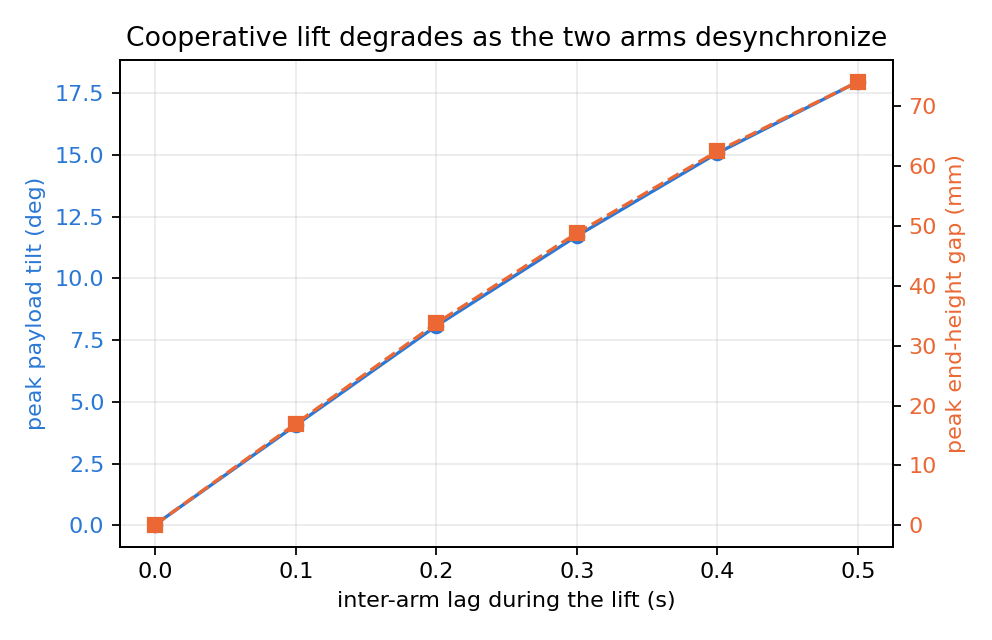
\includegraphics[width=0.78\linewidth]{figures/bimanual_desync_sweep.png}
\caption{The cooperative lift degrades smoothly as the two arms desynchronize: peak
payload tilt and the height gap between its two ends both grow with the inter-arm lag.}
\label{fig:sweep}
\end{figure}

\begin{figure}[t]
\centering
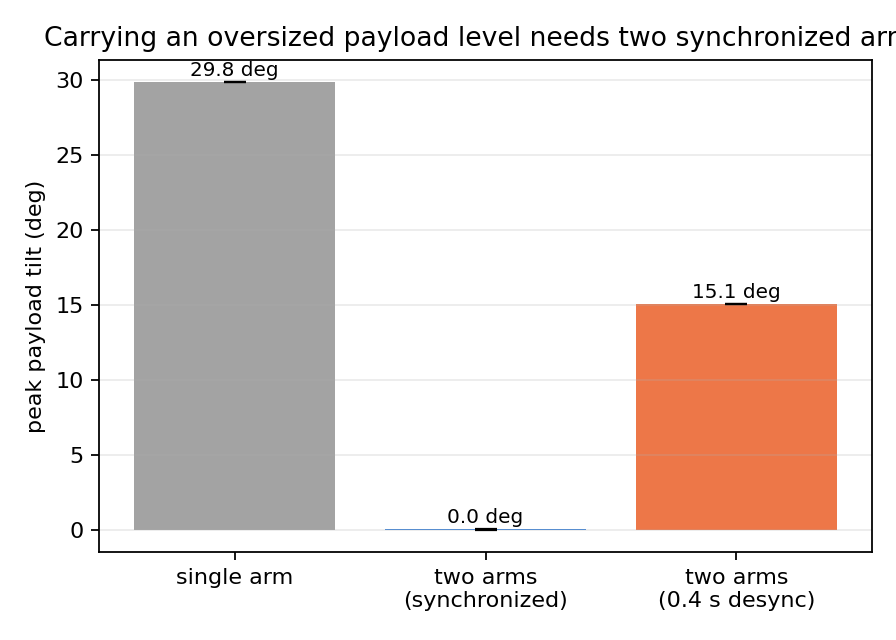
\includegraphics[width=0.66\linewidth]{figures/bimanual_tilt_comparison.png}
\caption{Peak payload tilt by condition. A single arm cannot keep the oversized payload
level; two synchronized arms keep it to within a degree; desynchronized arms see-saw it.}
\label{fig:tilt}
\end{figure}

\subsection{Lid close: an honest negative}
The lid-close result is the opposite of the intuition. One arm alone seats the lid essentially perfectly --- 0.9~mm off centre, the can displaced by 0.1~mm --- because the table back-stops the can against the downward press; the second hand is simply not needed. Worse, the naive two-arm version fails (Table~\ref{tab:lid}): with both arms converging on the same small can, they contend for it and knock it 124~mm aside. The lesson is not that coordination is unhelpful but that a task only needs a second hand when the world cannot supply the missing constraint --- here the table already does.

\begin{table}[t]
\centering
\caption{Lid close: an apparent two-hand task that one hand does better.}
\label{tab:lid}
\begin{tabular}{lccc}
\hline
Condition & Lid off-centre (mm) & Can displaced (mm) & Seated? \\
\hline
One hand (can free-standing) & 0.9 & 0.1 & yes \\
Two hands (one holds the can) & 185.6 & 124.2 & no \\
\hline
\end{tabular}
\end{table}

\subsection{Vision-guided balancing}
Closing the loop through vision transforms the task. With the arms simply holding the tray at a fixed, nominally level pose, the ball rolls to the downhill rail and rests 68~mm off centre: a small, unmodelled tilt bias in the shared grasp is enough to lose it, and nothing corrects it. With the vision loop closed, the same bias is cancelled and the ball is held 3~mm from centre --- a 25$\times$ reduction --- indefinitely (Table~\ref{tab:balance}, Figure~\ref{fig:balance}). When a transient centre-of-mass shift is then applied, it drives the ball to a peak of 20~mm off centre, from which the controller recovers to within the re-centred band in 2.9~s and settles at 9~mm; the open loop has no such recovery. Balancing the ball is, like carrying the payload, a genuinely cooperative act --- but here the coordination is continuous and closed through perception rather than scripted in time.

\begin{table}[t]
\centering
\caption{Vision-guided cooperative balancing: ball offset from the tray centre
(lower is better).}
\label{tab:balance}
\begin{tabular}{lcc}
\hline
Condition & Settled offset (mm) & Behaviour \\
\hline
Open loop (level hold) & 68 & rolls to the rail \\
Closed loop (vision) & 3 & held at centre \\
Closed loop, CoM shift & 9 (peak 20) & rejected, re-centred \\
\hline
\end{tabular}
\end{table}

\begin{figure}[t]
\centering
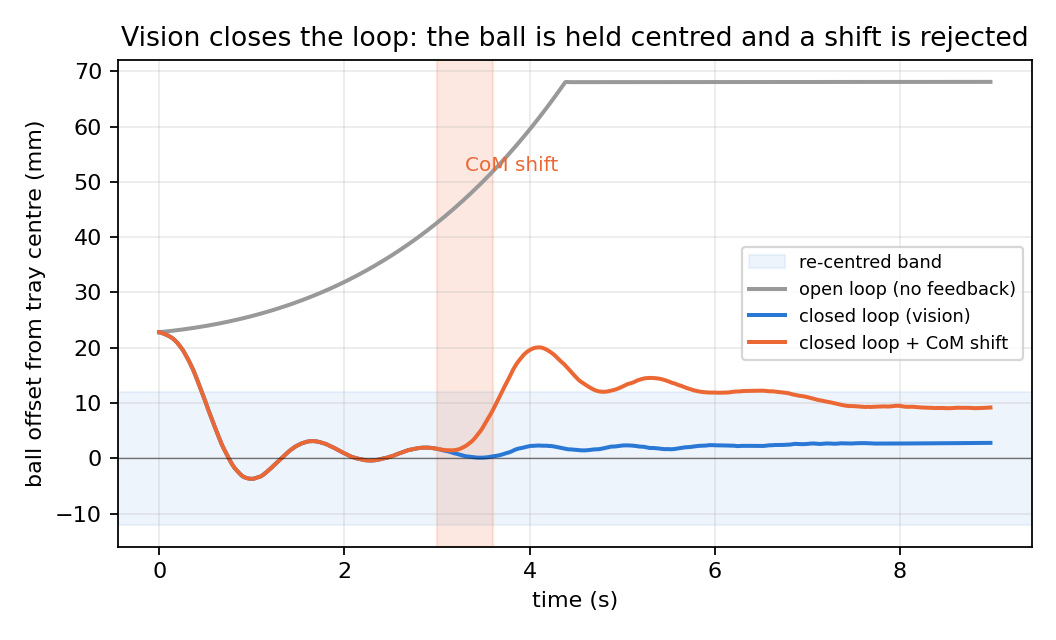
\includegraphics[width=0.82\linewidth]{figures/bimanual_ball_balance.png}
\caption{Vision-guided bimanual ball-balancing. Open loop (grey) the ball rolls to the
rail and stays; closed loop (blue) it is driven to the centre and held; under a transient
centre-of-mass shift (orange, shaded interval) it is knocked off centre and re-centred.}
\label{fig:balance}
\end{figure}

\section{Discussion}
Taken together the two tasks suggest a simple test for when a second hand is genuinely required: a second hand is necessary exactly when the task needs a constraint that neither the first hand nor the environment can supply. Carrying the oversized payload needs a second support the world cannot provide (there is no table under a payload in flight, and the object exceeds one gripper), so two hands are required --- and, being a closed chain, they must be coordinated in space and time. Seating the lid needs the can held still, but the table already supplies that against a vertical press, so one hand suffices. The coordination the genuine case demands is itself of a specific kind: tight spatio-temporal synchronization on a shared rigid body, distinct from the looser role-differentiation (one holds, one acts) that the lid task would have needed had the world not helped.

The balancing task adds a third kind of coordination to this picture: continuous, closed-loop, and driven by perception rather than by a clock. It also surfaces a property of closed-chain bimanual control worth stating plainly --- that the stability of two stiff position-controlled arms on a shared rigid body depends not on where they hold it but on how fast they are allowed to change their hold. A static cooperative grasp is stable; the same grasp driven by an unrate-limited controller is not. The joint-space slew limit that resolves this is a one-line change with an outsized effect, and it is the kind of detail that separates a controller that works in a figure from one that runs indefinitely.

\section{Limitations and Future Work}
\begin{itemize}

\item Simulation only. The dynamics, contacts and friction are idealised; a sim-to-real study with domain randomisation is the natural next step, as it is for the underlying single-arm platform.

\item A third genuinely two-hand regime --- handover across a partitioned workspace --- is identified but not completed here: it exposed a reach limitation of one arm at the far side of the shared centre under load, which a workspace-management and reachability-aware planning layer should resolve.

\item Screw (threaded) lid closing, which genuinely needs counter-torque and hence two hands, is left to future work because it requires continuous rotational contact and finger regrasping that rigid-body position control does not capture cleanly.

\item The balancing tray is short, so the controller rejects a slowly developing centre-of-mass shift but not a sharp impulsive shove, which carries the ball across the small workspace to the rail before the loop can respond. A longer beam, a faster effective control bandwidth, or an impedance rather than position inner loop would widen the class of disturbances rejected; the present result is deliberately the robust, reproducible one.

\item The balance loop regulates a single tilt axis against a scalar ball offset; full tray-pose stabilisation (both tilt axes and height) against a two-dimensional visual measurement of the payload is a natural generalisation.

\item The two arms do not yet share a collision-avoidance layer for arbitrarily overlapping reach; the present tasks keep each arm's working volume largely separate. A reservation-based deconfliction layer is the clear extension for dense shared-workspace operation.

\end{itemize}

\section{Conclusion}
We built a shared-workspace dual-arm testbed as a faithful extension of a validated single-arm platform, and used it to measure, rather than assume, bimanual coordination. Two synchronized arms carry an oversized payload level to within a degree where one arm cannot, and performance degrades smoothly and measurably as the arms are desynchronized --- a clean, quantitative coordination result. At the same time, a canonical ``two-hand'' task, closing a lid, turns out to need only one hand once the environment is allowed to help. The second finding disciplines the first: a second hand earns its place only when it supplies a constraint nothing else can, and when it does, the coordination it demands can be stated, measured, and designed for. Finally, closing the loop through the platform's own camera lets the two arms balance a ball on a tray they jointly hold, cancelling the grasp's tilt bias and rejecting a centre-of-mass shift --- extending the study from scripted, feed-forward coordination to continuous, perception-driven cooperation, and showing that the stability of such a closed chain hinges on rate-limiting how quickly the arms revise their shared hold.


\begin{thebibliography}{8}
\bibitem{smith} Smith, C., Karayiannidis, Y., et al.: Dual arm manipulation --- a survey.
Robotics and Autonomous Systems 60(10), 1340--1353 (2012)
\bibitem{caccavale} Caccavale, F., Uchiyama, M.: Cooperative manipulation. In: Springer
Handbook of Robotics, pp. 989--1006. Springer (2016)
\bibitem{hutchinson} Hutchinson, S., Hager, G.D., Corke, P.I.: A tutorial on visual servo
control. IEEE Trans. Robotics and Automation 12(5), 651--670 (1996)
\bibitem{todorov} Todorov, E., Erez, T., Tassa, Y.: MuJoCo: A physics engine for
model-based control. In: IEEE/RSJ IROS, pp. 5026--5033 (2012)
\bibitem{kulkarni} Kulkarni, Y.: Does fixed mean occluded? A cross-validated benchmark of
eye-in-hand vs. fixed-camera baselines for robotic manipulation. Preprint (2026)
\end{thebibliography}
\end{document}
